% REV01 Sun 28 Mar 2021 09:52:23 WIB
% START Fri 26 Mar 2021 17:22:59 WIB

\chapter{ON THE LOOK OUT}

In these times of ours, though concerning the exact year there is no
need to be precise, a boat of dirty and disreputable appearance,
with two figures in it, floated on the Thames, between Southwark
bridge which is of iron, and London Bridge which is of stone, as an
autumn evening was closing in.


\includegraphics[scale=2.3]{01-01-01}

The figures in this boat were those of a strong man with ragged
grizzled hair and a sun-browned face, and a dark girl of nineteen or
twenty, sufficiently like him to be recognizable as his daughter.
The girl rowed, pulling a pair of sculls very easily; the man, with
the rudder-lines slack in his hands, and his hands loose in his
waistband, kept an eager look out. He had no net, hook, or line,
and he could not be a fisherman; his boat had no cushion for a
sitter, no paint, no inscription, no appliance beyond a rusty
boathook and a coil of rope, and he could not be a waterman; his
boat was too crazy and too small to take in cargo for delivery, and
he could not be a lighterman or river-carrier; there was no clue to
what he looked for, but he looked for something, with a most intent
and searching gaze. The tide, which had turned an hour before,
was running down, and his eyes watched every little race and eddy
in its broad sweep, as the boat made slight head-way against it, or
drove stern foremost before it, according as he directed his
daughter by a movement of his head. She watched his face as
earnestly as he watched the river. But, in the intensity of her look
there was a touch of dread or horror.

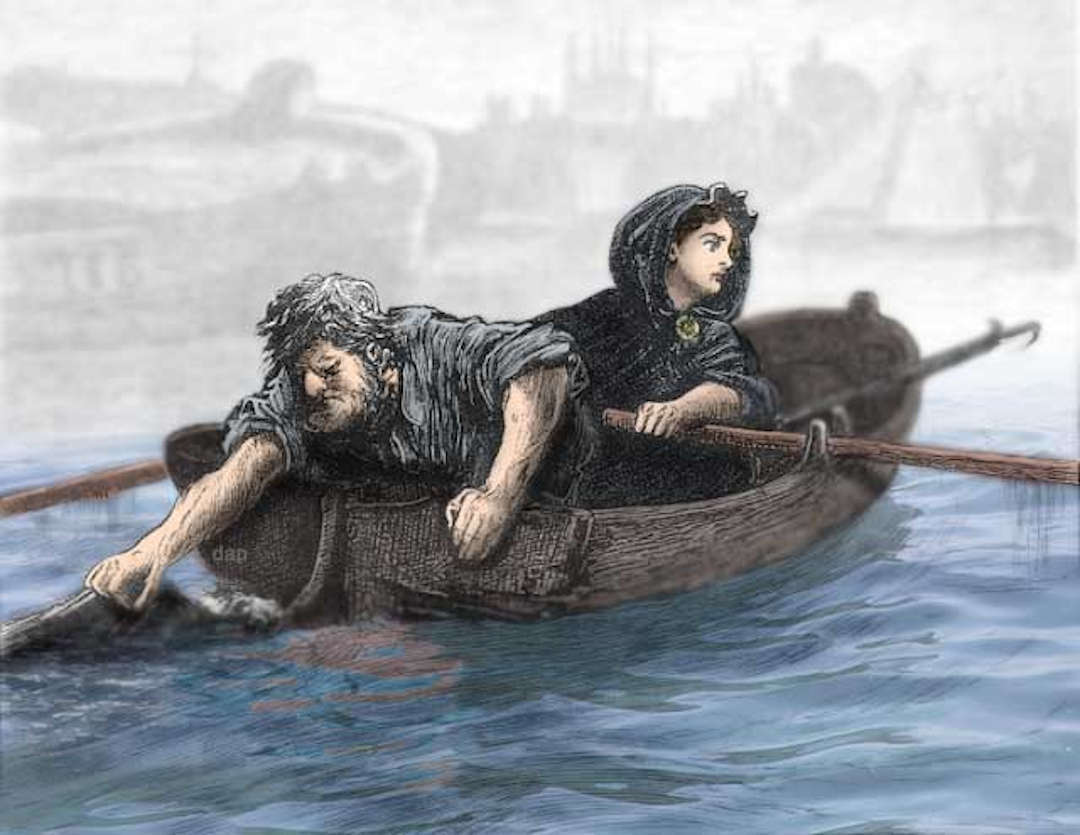
\includegraphics[scale=0.42]{01-01-02}

Allied to the bottom of the river rather than the surface, by reason
of the slime and ooze with which it was covered, and its sodden
state, this boat and the two figures in it obviously were doing
something that they often did, and were seeking what they often
sought. Half savage as the man showed, with no covering on his
matted head, with his brown arms bare to between the elbow and
the shoulder, with the loose knot of a looser kerchief lying low on
his bare breast in a wilderness of beard and whisker, with such
dress as he wore seeming to be made out of the mud that begrimed
his boat, still there was a business-like usage in his steady gaze.
So with every litle action of the girl, with every turn of her wrist,
perhaps most of all with her look of dread or horror; they were
things of usage.

'Keep her out, Lizzie. Tide runs strong here. Keep her well afore
the sweep of it.'

Trusting to the girl's skill and making no use of the rudder, he eyed
the coming tide with an absorbed attention. So the girl eyed him.
But, it happened now, that a slant of light from the setting sun
glanced into the bottom of the boat, and, touching a rotten stain
there which bore some resemblance to the outline of a muffled
human form, coloured it as though with diluted blood. This caught
the girl's eye, and she shivered.

'What ails you?' said the man, immediately aware of it, though so
intent on the advancing waters; 'I see nothing afloat.'

The red light was gone, the shudder was gone, and his gaze, which
had come back to the boat for a moment, travelled away again.
Wheresoever the strong tide met with an impediment, his gaze
paused for an instant. At every mooring-chain and rope, at every
stationery boat or barge that split the current into a broad-arrowhead,
at the offsets from the piers of Southwark Bridge, at the
paddles of the river steamboats as they beat the filthy water, at the
floating logs of timber lashed together lying off certain wharves,
his shining eyes darted a hungry look. After a darkening hour or
so, suddenly the rudder-lines tightened in his hold, and he steered
hard towards the Surrey shore.

Always watching his face, the girl instantly answered to the action
in her sculling; presently the boat swung round, quivered as from a
sudden jerk, and the upper half of the man was stretched out over
the stern.

The girl pulled the hood of a cloak she wore, over her head and
over her face, and, looking backward so that the front folds of this
hood were turned down the river, kept the boat in that direction
going before the tide.
Until now, the boat had barely held her own,
and had hovered about one spot; but now, the banks changed
swiftly, and the deepening shadows and the kindling lights of
London Bridge were passed, and the tiers of shipping lay on either
hand.

It was not until now that the upper half of the man came back into
the boat. His arms were wet and dirty, and he washed them over
the side. In his right hand he held something, and he washed that
in the river too.
It was money.
He chinked it once, and he blew
upon it once, and he spat upon it once,--'for luck,' he hoarsely said
--before he put it in his pocket.

'Lizzie!'

The girl turned her face towards him with a start, and rowed in silence.
Her face was very pale.
He was a hook-nosed man, and
with that and his bright eyes and his ruffled head, bore a certain
likeness to a roused bird of prey.

'Take that thing off your face.'

She put it back.

'Here! and give me hold of the sculls. I'll take the rest of the spell.'

'No, no, father! Father!--I cannot sit so near it!' No!
I can't indeed.

He was moving towards her to change places, but her terrified
expostulation stopped him and he resumed his seat.

‘What hurt can it do you?’

‘None, none. But I cannot bear it.’

‘It’s my belief you hate the sight of the very river.’

‘I--I do not like it, father.’

‘As if it wasn’t your living! As if it wasn’t meat and drink to you!’

At these latter words the girl shivered again, and for a moment paused
in her rowing, seeming to turn deadly faint. It escaped his attention,
for he was glancing over the stern at something the boat had in tow.

‘How can you be so thankless to your best friend, Lizzie? The very
fire that warmed you when you were a babby, was picked out of the river
alongside the coal barges. The very basket that you slept in, the tide
washed ashore. The very rockers that I put it upon to make a cradle
of it, I cut out of a piece of wood that drifted from some ship or
another.’

Lizzie took her right hand from the scull it held, and touched her
lips with it, and for a moment held it out lovingly towards him: then,
without speaking, she resumed her rowing, as another boat of similar
appearance, though in rather better trim, came out from a dark place and
dropped softly alongside.

‘In luck again, Gaffer?’ said a man with a squinting leer, who sculled
her and who was alone, ‘I know’d you was in luck again, by your wake as
you come down.’

‘Ah!’ replied the other, drily. ‘So you’re out, are you?’

‘Yes, pardner.’

There was now a tender yellow moonlight on the river, and the new comer,
keeping half his boat’s length astern of the other boat looked hard at
its track.

‘I says to myself,’ he went on, ‘directly you hove in view, yonder’s
Gaffer, and in luck again, by George if he ain’t! Scull it is,
pardner--don’t fret yourself--I didn’t touch him.’ This was in answer
to a quick impatient movement on the part of Gaffer: the speaker at the
same time unshipping his scull on that side, and laying his hand on the
gunwale of Gaffer’s boat and holding to it.

‘He’s had touches enough not to want no more, as well as I make him
out, Gaffer! Been a knocking about with a pretty many tides, ain’t he
pardner? Such is my out-of-luck ways, you see! He must have passed me
when he went up last time, for I was on the lookout below bridge here. I
a’most think you’re like the wulturs, pardner, and scent ‘em out.’

He spoke in a dropped voice, and with more than one glance at Lizzie who
had pulled on her hood again. Both men then looked with a weird unholy
interest in the wake of Gaffer’s boat.

‘Easy does it, betwixt us. Shall I take him aboard, pardner?’

‘No,’ said the other. In so surly a tone that the man, after a blank
stare, acknowledged it with the retort:

‘--Arn’t been eating nothing as has disagreed with you, have you,
pardner?’

‘Why, yes, I have,’ said Gaffer. ‘I have been swallowing too much of
that word, Pardner. I am no pardner of yours.’

‘Since when was you no pardner of mine, Gaffer Hexam Esquire?’

‘Since you was accused of robbing a man. Accused of robbing a live man!’
said Gaffer, with great indignation.

‘And what if I had been accused of robbing a dead man, Gaffer?’

‘You COULDN’T do it.’

‘Couldn’t you, Gaffer?’

‘No. Has a dead man any use for money? Is it possible for a dead man to
have money? What world does a dead man belong to? ‘Tother world. What
world does money belong to? This world. How can money be a corpse’s? Can
a corpse own it, want it, spend it, claim it, miss it? Don’t try to go
confounding the rights and wrongs of things in that way. But it’s worthy
of the sneaking spirit that robs a live man.’

‘I’ll tell you what it is--.’

‘No you won’t. I’ll tell you what it is. You got off with a short time
of it for putting your hand in the pocket of a sailor, a live sailor.
Make the most of it and think yourself lucky, but don’t think after
that to come over ME with your pardners. We have worked together in time
past, but we work together no more in time present nor yet future. Let
go. Cast off!’

‘Gaffer! If you think to get rid of me this way--.’

‘If I don’t get rid of you this way, I’ll try another, and chop you over
the fingers with the stretcher, or take a pick at your head with the
boat-hook. Cast off! Pull you, Lizzie. Pull home, since you won’t let
your father pull.’

Lizzie shot ahead, and the other boat fell astern. Lizzie’s father,
composing himself into the easy attitude of one who had asserted the
high moralities and taken an unassailable position, slowly lighted a
pipe, and smoked, and took a survey of what he had in tow. What he had
in tow, lunged itself at him sometimes in an awful manner when the boat
was checked, and sometimes seemed to try to wrench itself away, though
for the most part it followed submissively. A neophyte might have
fancied that the ripples passing over it were dreadfully like faint
changes of expression on a sightless face; but Gaffer was no neophyte
and had no fancies.

